%% ****** Start of file aiptemplate.tex ****** %
%%
%%   This file is part of the files in the distribution of AIP substyles for REVTeX4.
%%   Version 4.1 of 9 October 2009.
%%
%!TEX encoding = UTF-8 Unicode
% This is a template for producing documents for use with 
% the REVTEX 4.1 document class and the AIP substyles.
% 
% Copy this file to another name and then work on that file.
% That way, you always have this original template file to use.

\documentclass[aip,notitlepage,reprint]{revtex4-1}
%\documentclass[reprint]{revtex4-1}

\usepackage{amsfonts}
\usepackage{amsmath}
\usepackage{amssymb}
\usepackage{booktabs}
\usepackage{caption}
\usepackage{color}
\usepackage{comment}
\usepackage{graphicx}
\usepackage{hyperref}
%\usepackage[utf8]{inputenc} % allows using accents directly in text, like ÔøΩ
\usepackage{subfig}
\usepackage{xspace}


\captionsetup{justification=raggedright,
singlelinecheck=false
}

\newcommand{\pygbe}{\texttt{PyGBe}\xspace}
\newcommand{\gb}{{\small G\,B1\,D4$^\prime$}\xspace}
\newcommand{\ig}{{\small IgG}}
\newcommand{\pdb}{{\small PDB}\xspace}
\newcommand{\gmres}{\textsc{gmres}\xspace}
\newcommand{\bem}{\textsc{bem}\xspace}
\newcommand{\ses}{\textsc{ses}\xspace}
\newcommand{\sam}{\textsc{sam}}
\newcommand{\gpu}{\textsc{gpu}}
\newcommand{\cpu}{\textsc{cpu}}
\newcommand{\apbs}{\textsc{apbs}\xspace}
\newcommand{\nvidia}{\textsc{nvidia}\xspace}
\newcommand{\msms}{\texttt{\textsc{msms}}\xspace}
\newcommand{\amber}{\texttt{\textsc{amber}}\xspace}
\newcommand{\ccby}{\textsc{cc-by}\xspace}

\graphicspath{{figs/}} %  PATH to figure files-- change to ./ for submission



\begin{document}

% Use the \preprint command to place your local institutional report number 
% on the title page in preprint mode.
% Multiple \preprint commands are allowed.
%\preprint{}

\title{Probing protein orientation near charged nanosurfaces for simulation-assisted biosensor design} 


% Explanatory text should go in the []'s, 
% actual e-mail address or url should go in the {}'s for \email and \homepage.
% \affiliation command applies to all authors since the last \affiliation command. 
% The \affiliation command should follow the other information.

\author{Christopher D. Cooper}
\email[]{cdcooper@bu.edu,christopher.cooper@usm.cl}
%\thanks{}
\affiliation{Department of Mechanical Engineering, Boston University, Boston, MA.}
\affiliation{Mechanical Engineering, Universidad T\'ecnica Federico Santa Mar\'ia, Valpara\'iso, Chile.}
% Note:
%At FINAL paper stage, move USM to \affiliation instead instead of \altaffiliation
%\affiliation{Department of Mechanical Engineering, Universidad T\'ecnica Federico Santa Mar\'ia, Valpara\'iso, Chile}

\author{Natalia C. Clementi}
\email[]{ncclementi@gwu.edu}
\affiliation{Department of Mechanical \& Aerospace Engineering, The George Washington University, Washington, DC.}

\author{Lorena A. Barba}
\email[]{labarba@gwu.edu}
\homepage[]{http://lorenabarba.com/}
\affiliation{Department of Mechanical \& Aerospace Engineering, The George Washington University, Washington, DC.}

% Collaboration name, if desired (requires use of superscriptaddress option in \documentclass). 
% \noaffiliation is required (may also be used with the \author command).
%\collaboration{}
%\noaffiliation

%\date{\today}

\maketitle %\maketitle must follow title, authors, abstract and \pacs

\begin{center}
\textbf{Supplementary Material}
\end{center}
For the main result in the paper, looking at the orientation of \ig 2a near a surface with charge $\sigma=0.1$C/m$^2$ immersed in a solvent with 37mM of salt, we show here the contribution of each energy component to the probability distribution.
We studied the contribution of the solvation and surface energies to the orientation probability distribution to show that the orientation mechanism is guided by the solvation energy in this case.
Fig.~\ref{fig:supp} shows the probability distribution computed in three ways: using the total energy (Fig.~\ref{fig:full}), neglecting the surface energy (Fig.~\ref{fig:solv}), and neglecting the solvation energy (Fig.~\ref{fig:surf}). 
Both the angle combination of the preferred orientation and the probability magnitude are similar in Fig.~\ref{fig:solv} and Fig.~\ref{fig:full}, indicating that the influence of neglecting the surface energy is small.
Hence, the orientation of \ig 2a under these conditions is dominated by the solvation energy.


\begin{figure} 
   \centering
   \subfloat[Probability distribution with the total energy.]{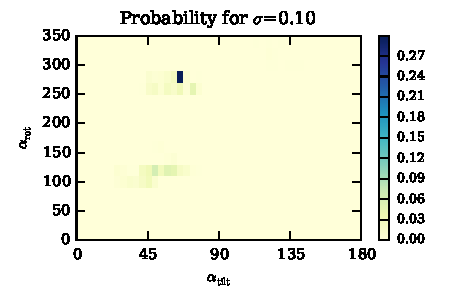
\includegraphics[width=0.43\textwidth]{figs/supp_1.pdf} \label{fig:full}}\\
   \subfloat[Probability distribution neglecting the surface energy.]{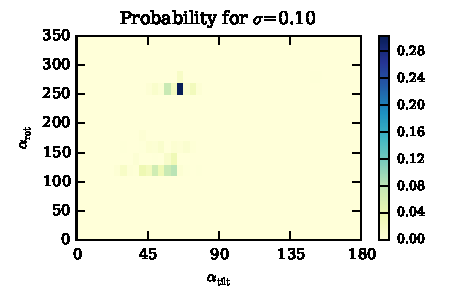
\includegraphics[width=0.43\textwidth]{figs/supp_2.pdf} \label{fig:solv}}\\
   \subfloat[Probability distribution neglecting the solvation energy.]{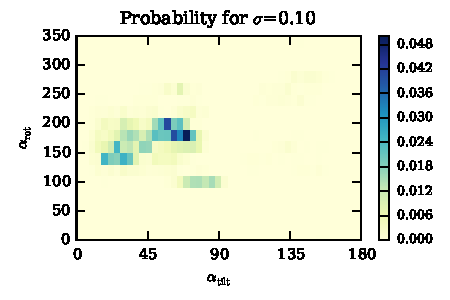
\includegraphics[width=0.40\textwidth]{figs/supp_3.pdf} \label{fig:surf}}
   \caption{}
   \label{fig:supp}
\end{figure}

\clearpage

\end{document}
